\documentclass{article}

% Language setting
% Replace `english' with e.g. `spanish' to change the document language
\usepackage[english]{babel}
\usepackage{color}
\usepackage{listings}

\definecolor{mygray}{rgb}{0.95, 0.95, 0.95}

\lstset{
    backgroundcolor=\color{mygray},
    language=bash,
    basicstyle=\ttfamily\small,
    commentstyle=
}

% Set page size and margins
% Replace `letterpaper' with `a4paper' for UK/EU standard size
\usepackage[letterpaper,top=2cm,bottom=2cm,left=3cm,right=3cm,marginparwidth=1.75cm]{geometry}

\setlength{\parindent}{0pt}

% Useful packages
\usepackage{amsmath}
\usepackage{graphicx}
\usepackage[colorlinks=true, allcolors=blue]{hyperref}

\graphicspath{{images}}

\title{CryptoLab Instruction}
\author{}

\begin{document}
\maketitle

\section{General Description}

CryptoLab is a system where students can practice cryptographic attacks and implement exchange policies. It consists of several machines running containerized (in Docker) apps. One machine that we call a \textbf{gateway} acts as a central access point for students. The other machines run \textbf{backend} server app (also Docker containerized) that do the actual work. Below is a diagram of the system's topology.

\begin{figure}[h]
    \centering
    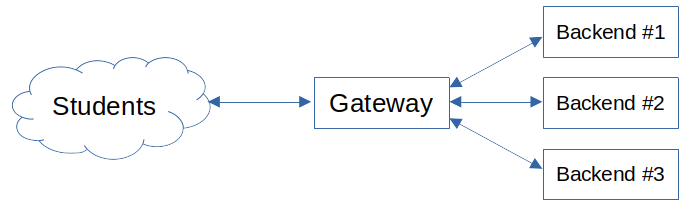
\includegraphics[width=0.8\textwidth]{scheme}
    \caption{Scheme of the system.}
\end{figure}

Students have access to the gateway machine alone. Gateway is listening 80 port, and students send their requests using HTTP protocol. Gateway runs a reverse proxy that acts as a load balancer for the backend machines. When the gateway receives a student's request, it redirects the request to one of the backend machines, which process the request and send back some response. This is a normal system's workflow. 

\section{Requirements}
\begin{enumerate}
    \item We need 3-4 computers running some Linux (preferably Ubuntu or similar) distro with sudo rights. 
    \item All machines must be accessible by IP address or by some name.
    \item One machine (the gateway) should be accessible by the name \texttt{cryptolab.csil.sfu.ca}. 
    \item All machines need Git, Docker, and SSH installed.
\end{enumerate}

\section{Installation}
\vspace{0.25cm}

First and foremost we must decide what machines are going to act as the gateway and the backends. This one is easy: the gateway has address \texttt{cryptolab.csil.sfu.ca}, while the backend machines can have any address. From now on we will refer to the address of the first backend machine by \texttt{ADDRESS-1}, \texttt{ADDRESS-2} is the address of the second backend machine, \texttt{ADDRESS-3} is the address of the third, etc.   

\vspace{1cm}

\paragraph{Setting up a backend} Log in via \texttt{SSH} or by other means into the first backend machine, and follow the steps below.

\vspace{0.25cm}

\textsc{Step 1}. Download the source code of the backend part of the system by executing this command in terminal
\begin{lstlisting}
$ git clone https://csil-git1.cs.surrey.sfu.ca/oomelche/crypto-backend.git
\end{lstlisting}
If the above command produces an error that the project could not be found or you're not authorized to clone the project, email the instructor. Next, change the working directory by running
\begin{lstlisting}
$ cd crypto-backend
\end{lstlisting}

\vspace{0.5cm}

\textsc{Step 2}. Make \texttt{build.sh} and \texttt{run.sh} scripts executable by running 
\begin{lstlisting}
$ chmod 700 build.sh run.sh stop.sh
\end{lstlisting}

\vspace{0.5cm}

\textsc{Step 3}. Build and containerize the backend's app
\begin{lstlisting}
$ ./build.sh
\end{lstlisting}
This process takes a while. At the end (if everything is ok) you should see a message like this
\begin{lstlisting}
Successfully built ac121ec2650f
Successfully tagged crypto/backend:latest
\end{lstlisting}
If you did get an error, investigate the error message, and fix the issue. At the time of writing this instruction, the building process went to completion with no problem.

\vspace{0.5cm}

\textsc{Step 4}. Run the app
\begin{lstlisting}
$ ./run.sh
\end{lstlisting}

\vspace{0.5cm}

\textsc{Step 5}. Check that the app is running by calling
\begin{lstlisting}
$ curl hhtp://localhost:8888/heartbeat
\end{lstlisting}
You should get the output like this
\begin{lstlisting}
{"cpu_count":4,"cpu_usage (%)":12.5,"current-time":"2023-01-29 05:25:09",
"host":"","is-alive":1,"mem_available":1102172160,"mem_total":10368090112,
"mem_usage (%)":89.4,"mem_used":8458248192,"server-id":"298c4",
"unix-epoch":1674969909.3859441}
\end{lstlisting}
This gives you some information about server the app is running at.

\vspace{0.5cm}
\textsc{Step 6}. Repeat all the above steps for the other backend machines as well.

\vspace{0.25cm}

\paragraph{Setting up a gateway} Log in into gateway machine via \texttt{SSH} or by other means, and follow the steps below.

\vspace{0.25cm}

\textsc{Step 1}. First, we need to make sure that the gateway ``sees'' the backend machines. Recall that we use \texttt{ADDRESS-1, ADDRESS-2,...} to denote an address of the corresponding backend machine. Run in terminal
\begin{lstlisting}
$ ping <ADDRESS-1>
\end{lstlisting}
For example, if the first backend machine has address 10.10.10.10, then run
\begin{lstlisting}
$ ping 10.10.10.10
\end{lstlisting}
and you should get something like
\begin{lstlisting}
PING 10.10.10.10 (10.10.10.10) 56(84) bytes of data.
64 bytes from 10.10.10.10: icmp_seq=1 ttl=119 time=7.52 ms
64 bytes from 10.10.10.10: icmp_seq=2 ttl=119 time=6.63 ms
64 bytes from 10.10.10.10: icmp_seq=3 ttl=119 time=7.04 ms
64 bytes from 10.10.10.10: icmp_seq=4 ttl=119 time=6.96 ms
\end{lstlisting}
If you do not see similar output, this signals that the gateway does not know how to reach the first backend machine. In that case email IT support to check the issue, since gateway and backend machines are expected to be reachable from each other. 

Run the same \texttt{ping} test for the other backend machines as well. All backend machines must be reachable from the gateway. 

\vspace{0.5cm}

\textsc{Step 2}. Next, we are going to add aliases for backends. That is open \texttt{/etc/hosts} file with \texttt{nano} editor by running (see Figure~\ref{fig:1} for an example what a \texttt{/etc/hosts} looks like in the \texttt{nano} editor)
\begin{lstlisting}[language=bash]
$ sudo nano /etc/hosts
\end{lstlisting}
enter user password, and you will see something similar to
\begin{figure}[h]
    \centering
    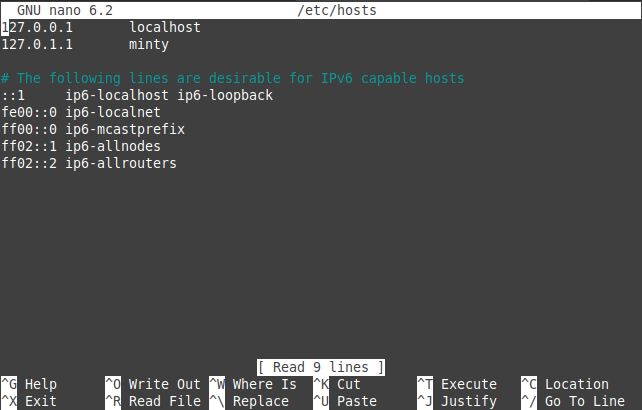
\includegraphics[width=0.8\textwidth]{nano-1}
    \caption{An example of what \texttt{/etc/hosts} looks like in \texttt{nano} editor.}
    \label{fig:1}
\end{figure}

Move cursor all the way down, and enter the following lines (the number of lines depends on the number of backend machines you have)
\begin{lstlisting}
<ADDRESS-1> crypto-01
<ADDRESS-2> crypto-02
<ADDRESS-3> crypto-03
\end{lstlisting}
The above lines will assign the first backend machine the name \texttt{crypto-01}, the second backend machine will be reachable by the name \texttt{crypto-02}, and finally the third backend machine will receive name \texttt{crypto-03}. If you have four (or more) backends, you can enter them here as well.

Next, press \texttt{Ctrl+X}. You will be asked whether you want to save the buffer. Press \texttt{Y} (for Yes), and then hit \texttt{Enter} to finally save the file. Verify that the changes were saved by running
\begin{lstlisting}[language=bash]
$ cat /etc/hosts
\end{lstlisting}
and you should see the newly added lines in the output of the above command.

As an example, suppose we have 3 backend machines with addresses 10.10.10.10, 10.10.10.20, and 10.10.10.30. Then we could assign them the aliases by changing the \texttt{/etc/hosts} to look like in the Figure~\ref{fig:3}.
\begin{figure}[!h]
    \centering
    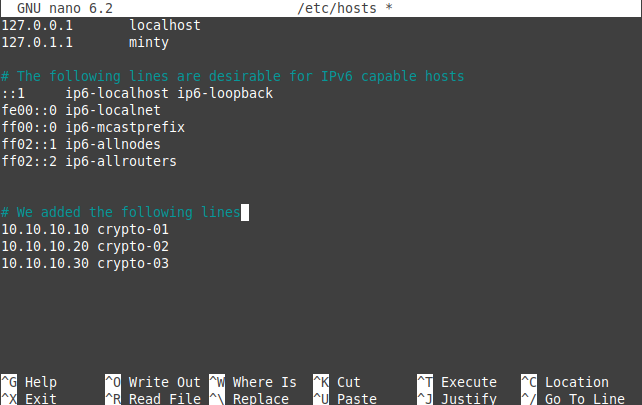
\includegraphics[width=0.8\textwidth]{nano-2}
    \caption{\texttt{/etc/hosts} file after we have added aliases for the backend machines.}
    \label{fig:3}
\end{figure}

After saving the file, and running the \texttt{cat /etc/hosts} command, you should see the lines similar to the ones below
\begin{lstlisting}
127.0.0.1	localhost
127.0.1.1	minty

# The following lines are desirable for IPv6 capable hosts
::1     ip6-localhost ip6-loopback
fe00::0 ip6-localnet
ff00::0 ip6-mcastprefix
ff02::1 ip6-allnodes
ff02::2 ip6-allrouters

# We added the following lines
10.10.10.10 crypto-01
10.10.10.20 crypto-02
10.10.10.30 crypto-03
\end{lstlisting}

\vspace{0.5cm}

\textsc{Step 3}. Now we need to verify that the aliases work. Run
\begin{lstlisting}[language=bash]
$ ping crypto-01
\end{lstlisting}
and check whether the gateway machine is able to send pings to the first backend machine called \texttt{crypto-01}. Run the same ping test for the other aliases.

\vspace{0.5cm} 

\textsc{Step 4}. The hardest part is done. Now run the following commands to clone the source code of the gateway into the current folder (if the link does not work, talk to the instructor)
\begin{lstlisting}[language=bash]
$ git clone https://csil-git1.cs.surrey.sfu.ca/oomelche/crypto-gateway.git
$ cd crypto-gateway
\end{lstlisting}
Next, we are going to edit gateway's configuration file. Run
\begin{lstlisting}
$ nano nginx.conf
\end{lstlisting}
to open \texttt{nginx.conf} file in the \texttt{nano} editor (see Figure~\ref{fig:2} for an example).
\begin{figure}[h!]
    \centering
    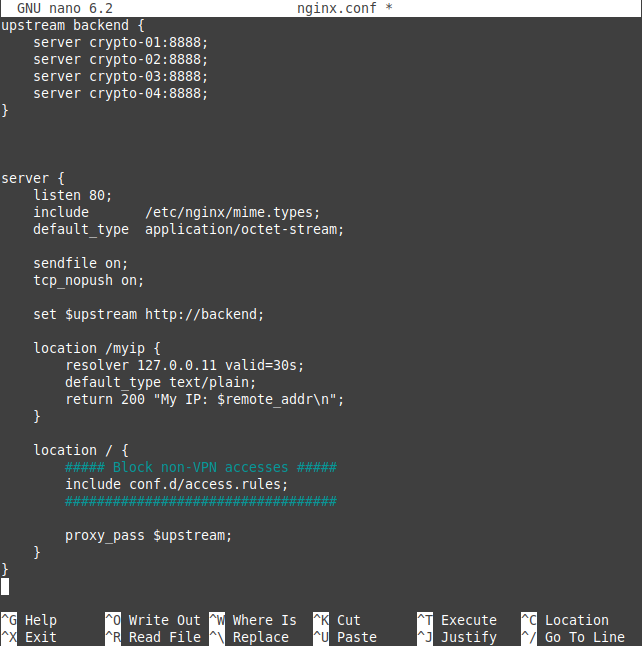
\includegraphics[width=0.8\textwidth]{nginx}
    \caption{\texttt{nginx.conf} file.}
        \label{fig:2}
\end{figure}
Observe the four lines \texttt{server crypto-0*:8888} of directives at the very top of the file. They tell the gateway app where to look for the backend machines.

Comment out unnecessary or add more lines like that if you have more than 4 backend machines, and you created aliases for them in the previous steps. To comment out, simply add \ \texttt{\#} \ a.k.a. the sharp symbol somewhere in front of the line, e.g.
\begin{lstlisting}
    server crypto-01:8888;
    server crypto-02:8888;
    server crypto-03:8888;
    # server crypto-04:8888;
\end{lstlisting}
comments out the last line. The number and aliases of the backend machines must match the number and aliases that you added into the \texttt{/etc/hosts} file in \textsc{Step 2}. Press \texttt{Ctrl+X}, and save the file.

\vspace{0.5cm}

\textsc{Step 5}. Now build/containerize the project by running
\begin{lstlisting}
$ chmod 700 build.sh run.sh run-it.sh stop.sh
$ ./build.sh
\end{lstlisting}
You will be asked if you want to stop all running containers. Enter \texttt{y} (for Yes), and it will start compiling the gateway app for you. It should not take too long to see the following output at the end
\begin{lstlisting}
Successfully tagged crypto/gateway:latest
\end{lstlisting}
If the gateway wasn't successfully packed into a container, then you will need to investigate what causes the trouble, since there could be many reasons. At the moment of writing this instruction the process goes smoothly with no issue (tested on several computers!).

\vspace{0.5cm}

\textsc{Step 6}. Now all is needed is to run the gateway app by executing
\begin{lstlisting}
$ ./run.sh
\end{lstlisting}
Verify that the gateway app is up and running by running the \texttt{curl} command
\begin{lstlisting}
$ curl http://localhost/myip
\end{lstlisting}
and you should get
\begin{lstlisting}
My IP: 127.0.0.1
\end{lstlisting}
If you did not get the above output, this signals that the gateway app didn't start up. You can check the problem by running the app in interactive mode by calling
\begin{lstlisting}
$ ./run-it.sh
\end{lstlisting}
and seeing what error message is produced. Hopefully, this will guide in solving the problem.

\vspace{0.5cm}

\textsc{Step 7}. Next, we need to run integration test. Connect to SFU VPN. Open your local browser and navigate to \texttt{http://cryptolab.csil.sfu.ca/heartbeat}. You should get an output like this~\footnote{\ Different browsers render JSON format in different ways, so you may get somewhat different output, but you should see a lot of information regardless how its rendered.}
\begin{lstlisting}
{
  "cpu_count": 4,
  "cpu_usage (%)": 26.8,
  "current-time": "2023-01-29 05:25:50",
  "host": "",
  "is-alive": 1,
  "mem_available": 1109323776,
  "mem_total": 10368090112,
  "mem_usage (%)": 89.3,
  "mem_used": 8455544832,
  "server-id": "298c4",
  "unix-epoch": 1674969950.1613266
}
\end{lstlisting}
Every time you request the above page, gateway sends request to a different backend. The backend's ID is displayed in the \texttt{server-id} field. Refresh the page several times, and count how many different \texttt{server-id}'s you get. The total number of different \texttt{server-id}'s should be the same as the number of backend servers.

Also check the \texttt{current-time} field of all the backends. It must be roughly the same every time you refresh the page. If you note that some backend's time is different from the others, fix that.
\end{document}